% request reply
\begin{frame}
    \begin{center}
        \vspace{1cm}
            \Huge \oran{Ejemplo}\\
            \Large \gray{Request - Reply}
    \end{center}
\end{frame}

\begin{frame}
    \frametitle{Ejemplo}
    \framesubtitle{Request Reply}
    \begin{center}
        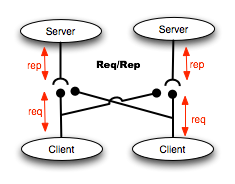
\includegraphics[width=0.4\textwidth]{img/request-reply}
    \end{center}
\end{frame}

\begin{frame}[fragile]
    \frametitle{Ejemplo}
    \framesubtitle{Request Reply - Server}

    \begin{python}
        import zmq
        import zmq
        context = zmq.Context()
        socket = context.socket(zmq.REP)
        socket.bind("tcp://127.0.0.1:5000")
        
        while True:
            msg = socket.recv()
            print "Got", msg
            socket.send(msg)
    \end{python}

\end{frame}


\begin{frame}[fragile]
    \frametitle{Ejemplo}
    \framesubtitle{Request Reply - Client}

    \begin{python}
        import zmq
        context = zmq.Context()
        socket = context.socket(zmq.REQ)
        socket.connect("tcp://127.0.0.1:5000")
        
        for i in range(10):
            msg = "msg %s" % i
            socket.send(msg)
            print "Sending", msg
            msg_in = socket.recv()
    \end{python}

\end{frame}


% publish subscriber
\begin{frame}
    \begin{center}
        \vspace{1cm}
            \Huge \oran{Ejemplo}\\
            \Large \gray{Publish Subscriber}
    \end{center}
\end{frame}

\begin{frame}
    \frametitle{Ejemplo}
    \framesubtitle{Publish Subscriber}
    \begin{center}
        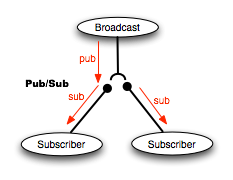
\includegraphics[width=0.4\textwidth]{img/publish-subscriber}
    \end{center}
\end{frame}

\begin{frame}[fragile]
    \frametitle{Ejemplo}
    \framesubtitle{Publish Subscriber - Server}

    \begin{python}
        import zmq
        from random import choice
        context = zmq.Context()
        socket = context.socket(zmq.PUB)
        socket.bind("tcp://127.0.0.1:5000")
        
        countries = ['netherlands','brazil','germany','portugal']
        events = ['yellow card', 'red card', 'goal', 'corner', 'foul']
        
        while True:
            msg = choice( countries ) +" "+ choice( events )
            print "->",msg
            socket.send( msg )
    \end{python}

\end{frame}


\begin{frame}[fragile]
    \frametitle{Ejemplo}
    \framesubtitle{Publish Subscriber - Client}

    \begin{python}
        import zmq
        
        context = zmq.Context()
        socket = context.socket(zmq.SUB)
        socket.connect("tcp://127.0.0.1:5000")
        socket.setsockopt(zmq.SUBSCRIBE, "netherlands")
        socket.setsockopt(zmq.SUBSCRIBE, "germany")
        
        while True:
            print  socket.recv()
    \end{python}

\end{frame}




% paired
\begin{frame}
    \begin{center}
        \vspace{1cm}
            \Huge \oran{Ejemplo}\\
            \Large \gray{Paired}
    \end{center}
\end{frame}

\begin{frame}
    \frametitle{Ejemplo}
    \framesubtitle{Paired}
    \begin{center}
        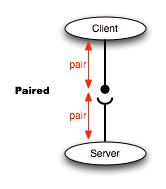
\includegraphics[width=0.4\textwidth]{img/paired}
    \end{center}
\end{frame}

\begin{frame}[fragile]
    \frametitle{Ejemplo}
    \framesubtitle{Paired - Server}

    \begin{python}
        import zmq
        context = zmq.Context()
        socket = context.socket(zmq.PAIR)
        socket.bind("tcp://127.0.0.1:5555")
        
        while True:
            msg = socket.recv()
            print "Got", msg
            socket.send(msg)
    \end{python}

\end{frame}


\begin{frame}[fragile]
    \frametitle{Ejemplo}
    \framesubtitle{Paired - Client}

    \begin{python}
        import zmq
        context = zmq.Context()
        socket = context.socket(zmq.PAIR)
        socket.connect("tcp://127.0.0.1:5555")
        
        for i in range(10):
            msg = "msg %s" % i
            socket.send(msg)
            print "Sending", msg
            msg_in = socket.recv()
    \end{python}

\end{frame}


% node coordination
\begin{frame}
    \begin{center}
        \vspace{1cm}
            \Huge \oran{Ejemplo}\\
            \Large \gray{Node Coordination}
    \end{center}
\end{frame}

\begin{frame}
    \frametitle{Ejemplo}
    \framesubtitle{Paired}
    \begin{center}
        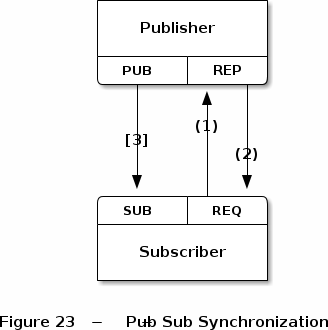
\includegraphics[width=0.4\textwidth]{img/nodecoord}
    \end{center}
\end{frame}



\begin{frame}
    \frametitle{Benchmarks}
    \begin{itemize}
        \item Ambiente:
        \begin{itemize}
            \item 2 Computadores, 8-core AMD Opteron 8356, 2.3GHz y 8-core Intel Xeon E5440, 2.83GHz
            \item Red: non-switched 10GbE network.
        \end{itemize}
        \item Pruebas:
        \begin{itemize}
            \item Envío de mensajes de tamaños:
             \begin{itemize}
                 \item 1, 2, 4, 8, 16, 32, ... , 32768 y 65536 bytes.
             \end{itemize}
        \end{itemize}
    \end{itemize}
\end{frame}

\begin{frame}
    \frametitle{Benchmarks}
    \framesubtitle{Latencia}
    \begin{itemize}
        \item 28.45 µs para mensajes de 1 byte (estable hasta 512B (33.08 us))
    \end{itemize}
    \begin{center}
        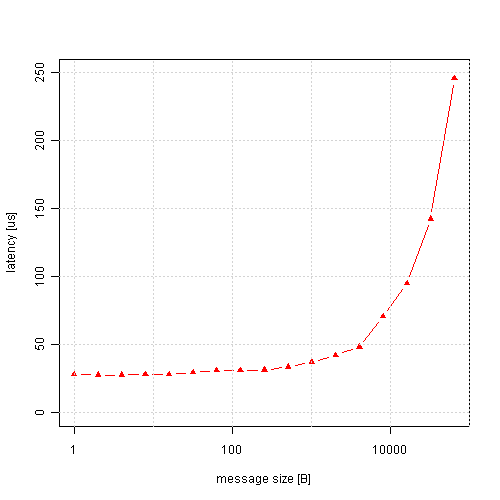
\includegraphics[width=0.5\textwidth]{img/latency}
    \end{center}
\end{frame}

\begin{frame}
    \frametitle{Benchmarks}
    \framesubtitle{Rendimiento}
    \begin{itemize}
        \item Máximo de 2.8 millones de mensajes por segundo (8 byte)
    \end{itemize}
    \begin{center}
        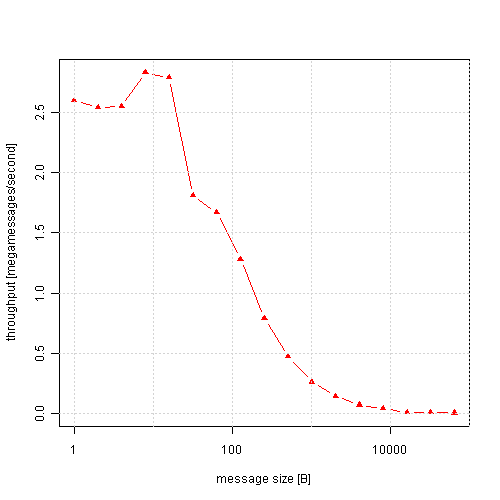
\includegraphics[width=0.5\textwidth]{img/throughput}
    \end{center}
\end{frame}

